%%%%%%%%%%%%%%%%%%%%%%%%%%%%%%%%%%%%%%
% LaTeX poster template
% Created by Nathaniel Johnston
% August 2009
% http://www.nathanieljohnston.com/2009/08/latex-poster-template/
%%%%%%%%%%%%%%%%%%%%%%%%%%%%%%%%%%%%%%

\documentclass[final]{beamer}
\usepackage[scale=1.24]{beamerposter}
\usepackage{graphicx}			% allows us to import images

%-----------------------------------------------------------
% Define the column width and poster size
% To set effective sepwid, onecolwid and twocolwid values, first choose how many columns you want and how much separation you want between columns
% The separation I chose is 0.024 and I want 4 columns
% Then set onecolwid to be (1-(4+1)*0.024)/4 = 0.22
% Set twocolwid to be 2*onecolwid + sepwid = 0.464
%-----------------------------------------------------------

\newlength{\sepwid}
\newlength{\onecolwid}
\newlength{\twocolwid}
\newlength{\threecolwid}
\setlength{\paperwidth}{48in}
\setlength{\paperheight}{36in}
\setlength{\sepwid}{0.024\paperwidth}
\setlength{\onecolwid}{0.22\paperwidth}
\setlength{\twocolwid}{0.464\paperwidth}
\setlength{\threecolwid}{0.708\paperwidth}
\setlength{\topmargin}{-0.5in}
\usetheme{confposter}
\usepackage{exscale}

%-----------------------------------------------------------
% The next part fixes a problem with figure numbering. Thanks Nishan!
% When including a figure in your poster, be sure that the commands are typed in the following order:
% \begin{figure}
% \includegraphics[...]{...}
% \caption{...}
% \end{figure}
% That is, put the \caption after the \includegraphics
%-----------------------------------------------------------

\usecaptiontemplate{
\small
\structure{\insertcaptionname~\insertcaptionnumber:}
\insertcaption}

%-----------------------------------------------------------
% Define colours (see beamerthemeconfposter.sty to change these colour definitions)
%-----------------------------------------------------------

\setbeamercolor{block title}{fg=ngreen,bg=white}
\setbeamercolor{block body}{fg=black,bg=white}
\setbeamercolor{block alerted title}{fg=white,bg=dblue!70}
\setbeamercolor{block alerted body}{fg=black,bg=dblue!10}

%-----------------------------------------------------------
% Name and authors of poster/paper/research
%-----------------------------------------------------------

\title{Punitive Measures: Because Finding a Good Pun is its own Reword}
\author{GROUP C - Amir Kashipazha, Brandon Boylan-Peck, Cathlyn Stone, Kenneth Hunter Wapman, Shantanu Karnwal}
\institute{CSCI 5622 (Machine Learning), University of Colorado Boulder}

%-----------------------------------------------------------
% Start the poster itself
%-----------------------------------------------------------

\begin{document}
\begin{frame}[t]
	\begin{columns}[t] % the [t] option aligns the column's content at the top
		%----------------------------------------------------------------------------------------
		\begin{column}{\sepwid}\end{column}			% empty spacer column
		%----------------------------------------------------------------------------------------
		\begin{column}{\onecolwid}

			\vspace{110mm}
			\begin{block}{Puns}
				{\large
					A \textbf{Pun} is form of wordplay in which a word\textquotesingle s multiple meanings or similar sounding words are used in a comedical manner. \\
					\vspace{40mm}
					Accurate identification and interpretation of puns would help improve human-computer communication, machine translation, and literary analysis.\\
					\vspace{40mm}
					There are many types of puns, but we focused on these two types:\\
						\\
					
					\begin{itemize}
						\item {\textbf{Homographic}: A pun involving two words whose spellings are the same but have different meanings.\\
								\textit{I used to be a banker but I lost \textbf{interest}.}}
						\item {\textbf{Heterographic}: A pun involves two or more words which sound alike but are spelled differently.\\
								\textit{Two construction workers had a \textbf{stairing} contest.}}
					\end{itemize}
					\vspace{40mm}
					We worked on two tasks: 
					\begin{itemize}
						\item {Pun \textbf{Detection}: determining whether a sentence is a pun or not}
						\item {Pun \textbf{Location}: identifying the word in a pun sentence which `makes' the pun}
					\end{itemize}
				}
			\end{block}
		\end{column}
		%----------------------------------------------------------------------------------------
		\begin{column}{\sepwid}\end{column} % Empty spacer column
		%----------------------------------------------------------------------------------------
		% center column (tasks)
		%----------------------------------------------------------------------------------------
		\begin{column}{\twocolwid}
			%----------------------------------------------------------------------------------------
			% top row
			%----------------------------------------------------------------------------------------
			\begin{columns}[t,totalwidth=\twocolwid] % Split up the two columns wide column
				%----------------------------------------------------------------------------------------
				% left column (description)
				%----------------------------------------------------------------------------------------
				\begin{column}{\onecolwid}\vspace{-.6in}
					\vspace{40mm}
					\begin{block}{Task 1 - Pun Detection}
						{\large 
							Pun detection is a binary classification problem: given a sentence, determine whether or not that sentence contains a pun. Given the binary nature of the solution space and the highly non-linear input space, machine learning seems to be a natural choice to detect puns.\\
							We have used three approaches for pun detection - 
							\begin{itemize}
							\item {\textbf{Naive Bayes classifier (Baseline)}}
							\item {\textbf{Recurrent Neural Network}}
							\item {\textbf{Feature Engineering based classifier}: We used the Stochastic Gradient Descent algorithm while combining different features like lesk algorithm, homophones, homonyms, antonyms, idioms, part of speech tagging.}
							\end{itemize}
						}
					\end{block}
				\end{column}
				%----------------------------------------------------------------------------------------
				% right column (images)
				%----------------------------------------------------------------------------------------
				\begin{column}{\onecolwid}\vspace{-.6in}
				
					\begin{SCfigure}
						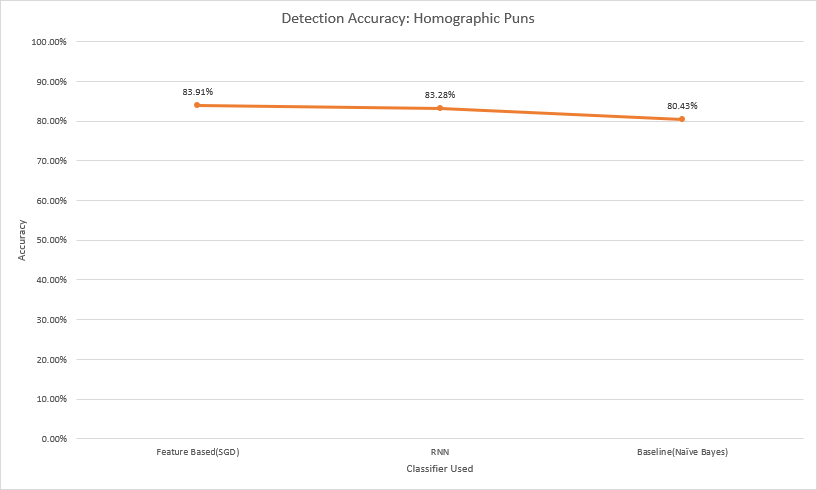
\includegraphics[width=0.85\textwidth]{HomographicDetection.png}\\
						\caption{Figure 1.1 - Pun Detection algorithm running on the Homographic Dataset.}
					\end{SCfigure}
					\\
					\vspace{20mm}
					\begin{SCfigure}
						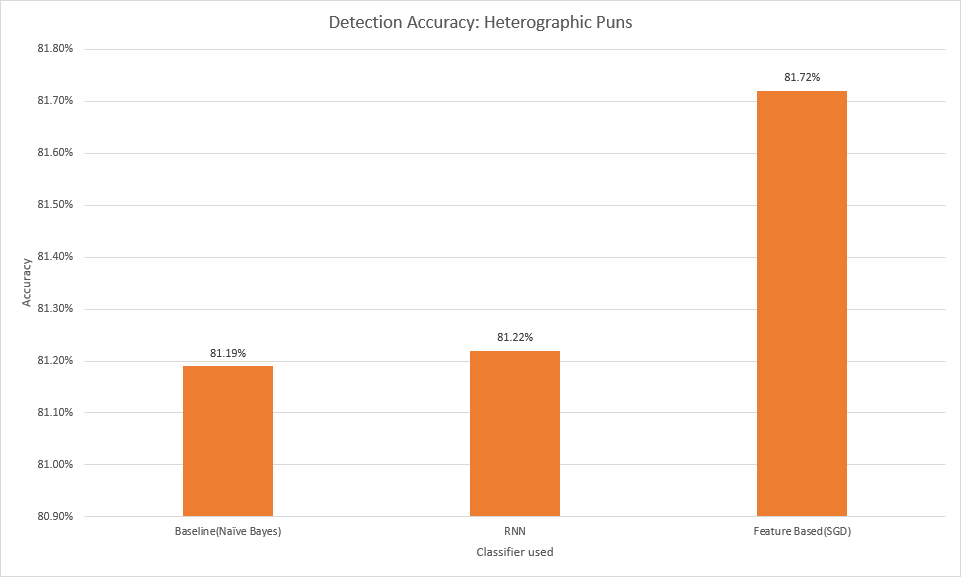
\includegraphics[width=0.85\textwidth]{HeterographicDetection.png}\\
						\caption{Figure 1.2 - Pun Detection algorithm running on the Heterographic Dataset.}
					\end{SCfigure}
				\end{column}
				%----------------------------------------------------------------------------------------
				% end top center column
				%----------------------------------------------------------------------------------------
			\end{columns}
			\begin{block}
				{.}
			\end{block}
			%----------------------------------------------------------------------------------------
			% bottom row
			%----------------------------------------------------------------------------------------
			\begin{columns}[t,totalwidth=\twocolwid]
				%----------------------------------------------------------------------------------------
				% left column
				%----------------------------------------------------------------------------------------
				\begin{column}{\onecolwid} % The second column within column 2 (column 2.2)

					\begin{SCfigure}
					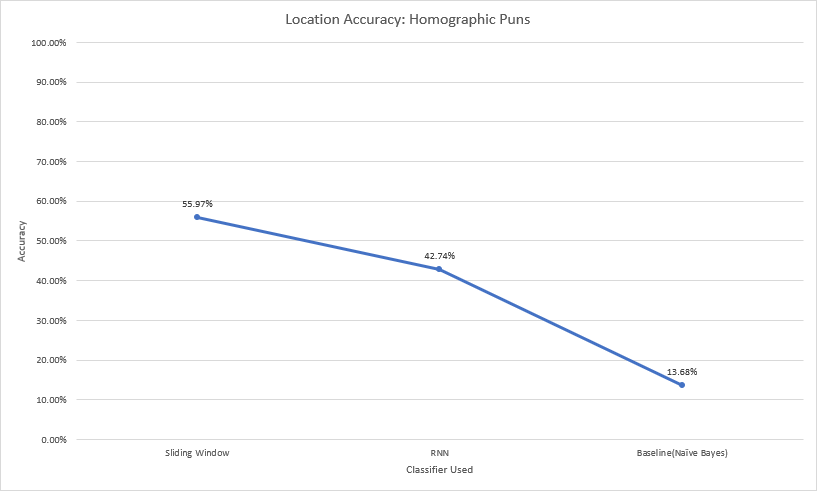
\includegraphics[width=0.85\textwidth]{HomographicLocation.png}\\
					\caption{Figure 2.1 - Pun Location algorithm running on the Homographic Dataset.}
					\end{SCfigure}
					\\
					\vspace{20mm}
					\begin{SCfigure}
					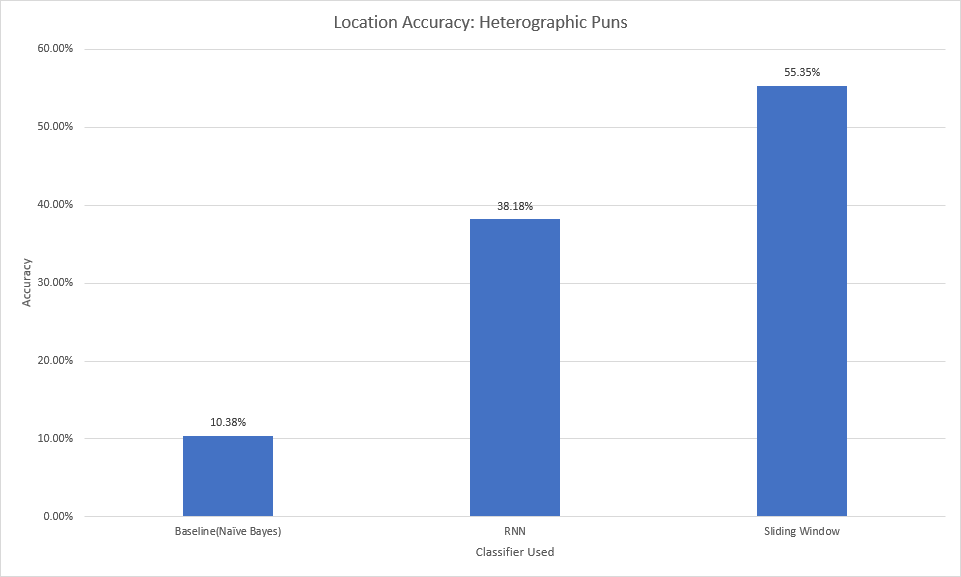
\includegraphics[width=0.85\textwidth]{HeterographicLocation.png}\\
					\caption{Figure 2.2 - Pun Location algorithm running on the Heterographic Dataset.}
					\end{SCfigure}
				\end{column} % End of column 2.2
				%----------------------------------------------------------------------------------------
				% right column
				%----------------------------------------------------------------------------------------
				\begin{column}{\onecolwid}
					\vspace{20mm}
					\begin{block}{Task 2 - Pun Location}
						{\large 
							The Pun locaton problem can be remodelled as: for each word in the sentence, determine the likelihood that that word is a pun given the rest of the sentence. Then, output the word which is most likely to be a pun based on the output of the previous search. \\
							We have used three approaches for pun detection - 
							\begin{itemize}
							\item {\textbf{Naive Bayes classifier (Baseline)}}
							\item {\textbf{Recurrent Neural Network} %: A homographic pun involves two words which are spelled the same but have different meanings.}
							}
							\item {\textbf{Sliding Window Based Classifier} : The sliding window classifier starts from the first word of the sentence and two words on either side to make a window of size five. Then it runs a max entropy classifier on this window, before sliding the window one word forward through the sentence. The block with highest entropy gives out the pun word.}
							\end{itemize}
							\\
						}
					\end{block}
				\end{column}
				\begin{column}{\sepwid}\end{column} % Empty spacer column
			\end{columns}
		\end{column}
		\begin{column}{\sepwid}\end{column} % Empty spacer column
		%----------------------------------------------------------------------------------------
		% rightmost column
		%----------------------------------------------------------------------------------------
		\begin{column}{\onecolwid}
            
			\begin{block}{Interactive Pun Detector \& Pun Locator}
				\large{
					We built a web application where a user can see the probability that a sentence is a homographic or heterographic pun as estimated by each algorithm we implemented.
				}

				\begin{SCfigure}
				\centering
				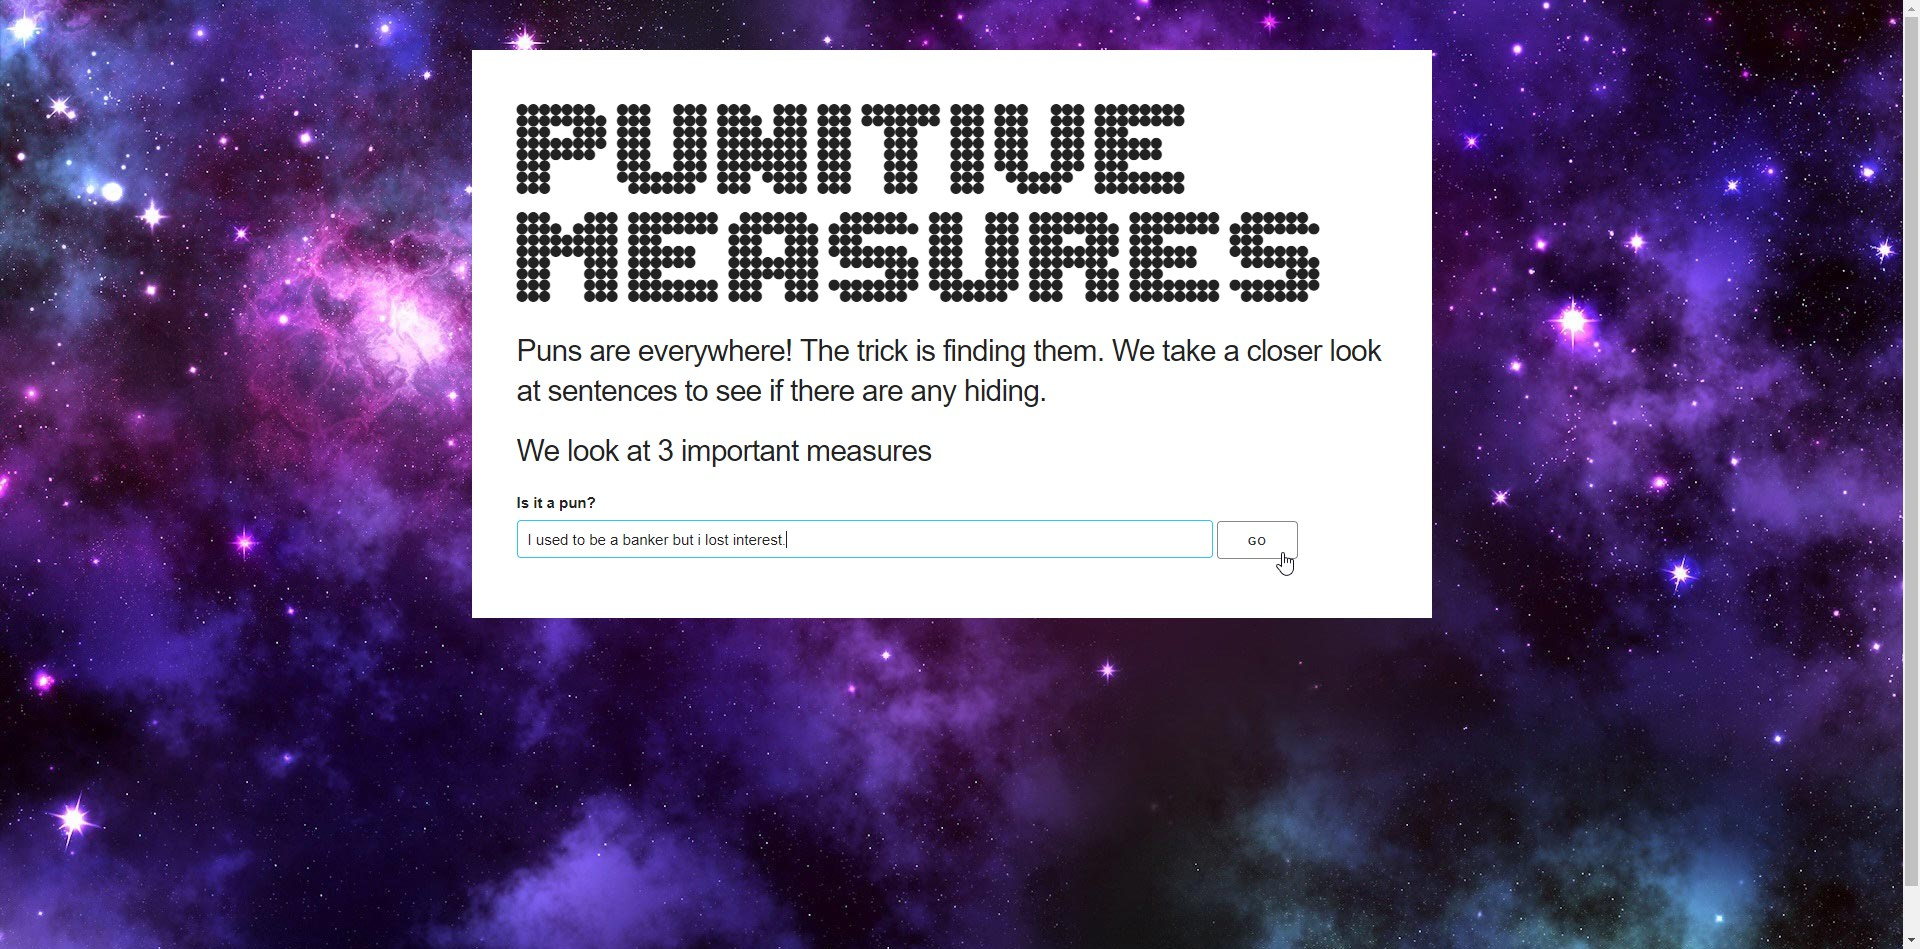
\includegraphics[width=0.75\textwidth]{UI_1.jpg}\\
				\caption{Figure 3.1 - Welcome Page.}
				\end{SCfigure}
				\\
				\vspace{20mm}
				\begin{SCfigure}
				\centering
				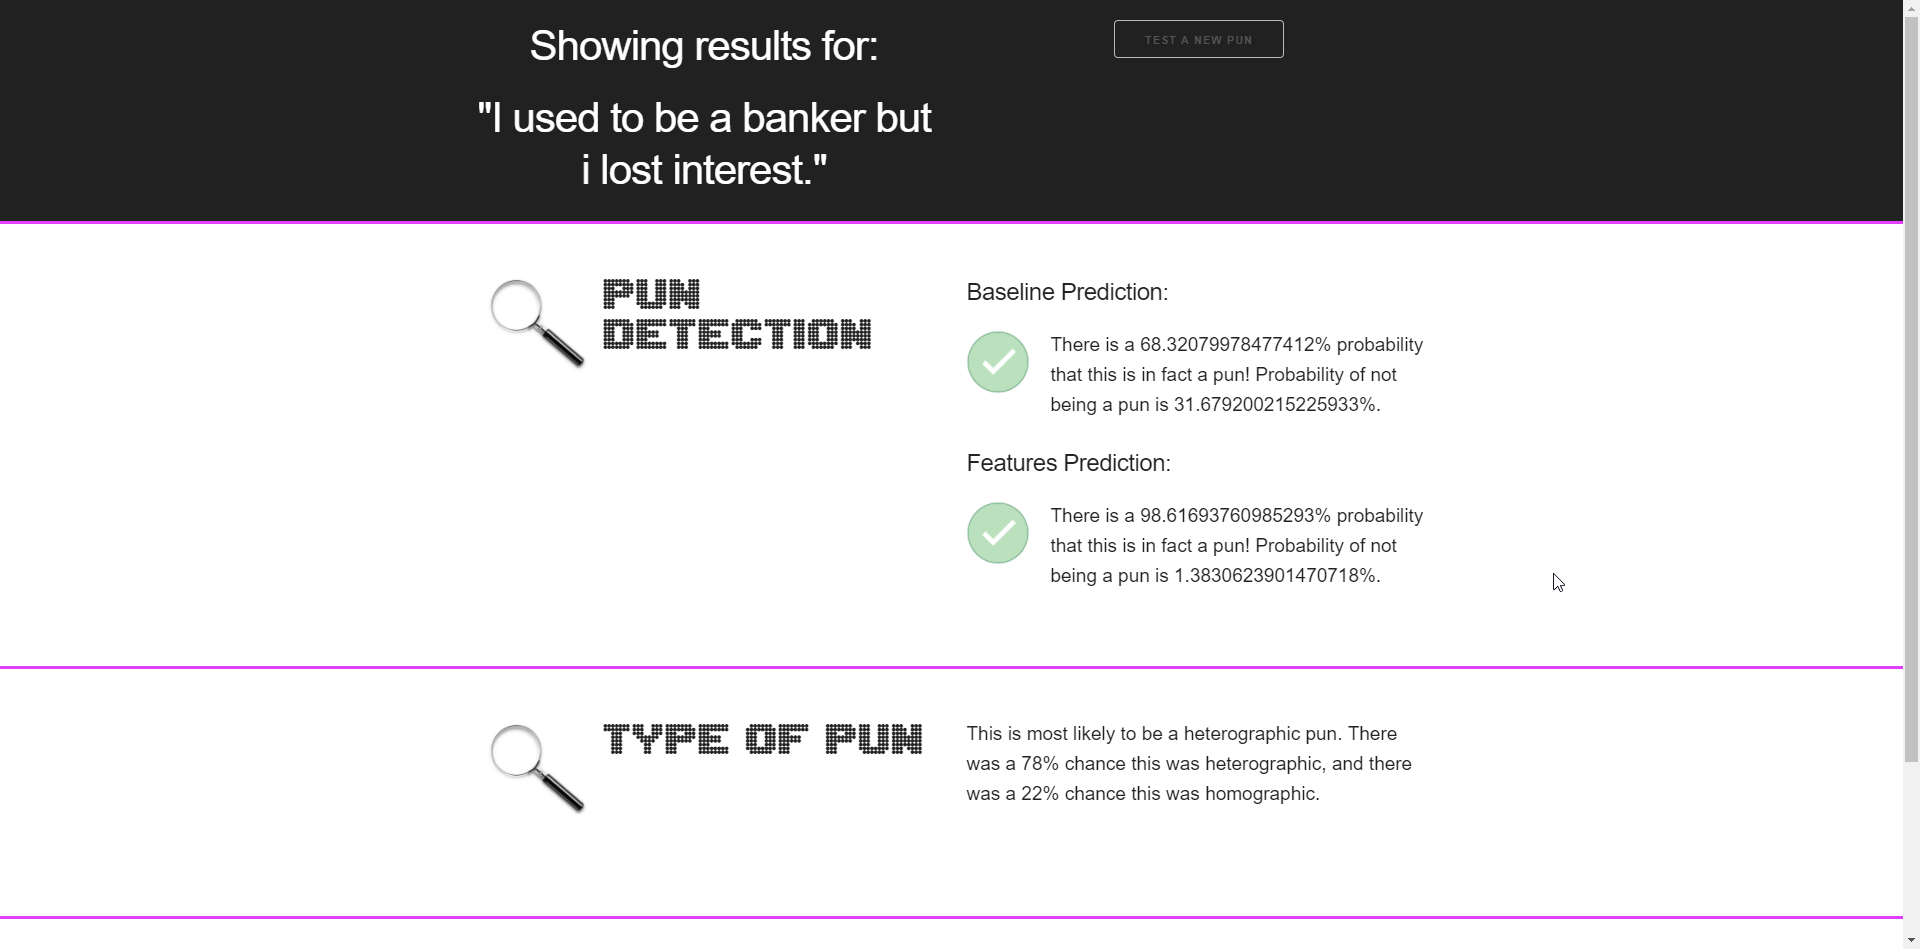
\includegraphics[width=0.75\textwidth]{UI_2.png}\\
				\centering
				\caption{Figure 3.2 - Analysis of the input sentence}
				\end{SCfigure}
			\end{block}
			\vspace{20mm}
            \begin{block}{Challenges}
            \end{block}
            \vspace{20mm}
            \begin{block}{How well did we do?}
            \end{block}
		\end{column}
		\begin{column}{\sepwid}\end{column}
	\end{columns}
\end{frame}
\end{document}
